\def\currentRootFolder{chapter/modelOfIntegratedRate}
\def\currentFigureFolder{\currentRootFolder/fig}
\newacronym{ssc}{SSC}{source and spectrum calculation}

\newcommand{\fermiConst}{G_\mathrm{F}}
\newcommand{\diffRate}{\frac{\d\Gamma(\Esource)}{\d \Esource}}
\newcommand{\nucMatrixElement}{M_\mathrm{nuc}}
\newcommand{\thetaFunc}{\Theta}

\newcommand{\nuMass}{m_\upnu}

\chapter{Mathematical Model of a KATRIN Measurement}
\label{sec:intSpecModel}
This chapter aims at deriving a mathematical expression for the integrated $\upbeta$-decay rate measured by KATRIN in order to be used in parameter inference.
\todo{Write chapter outline. Here are some useful sentences: In $\upbeta^-$ decay the released energy is distributed among the emitted electron and the anti-electron neutrino. }

\section{Differential \texorpdfstring{$\upbeta$}{Beta}-Decay Spectrum of Tritium}
\label{sec:intSpecModelDiffSpec}
\begin{figure}
	\centering
	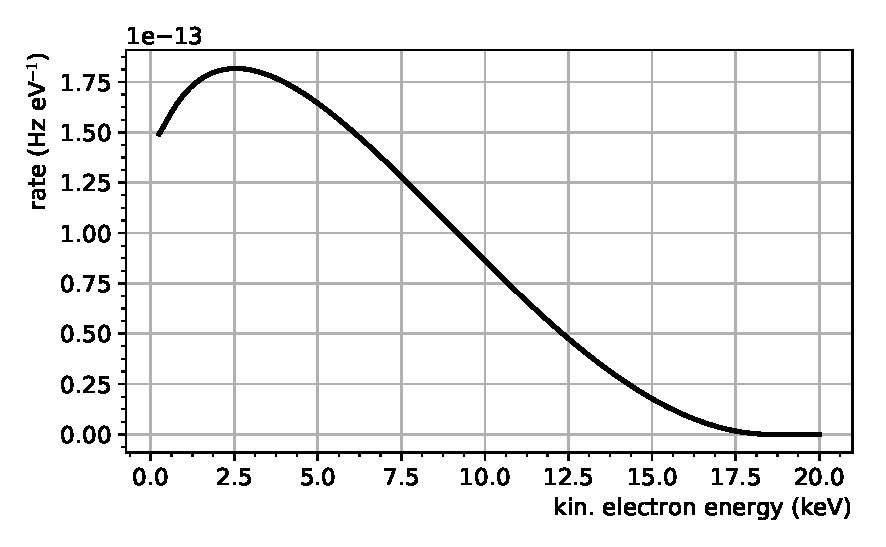
\includegraphics[width=\textwidth]{\currentFigureFolder/diffSpec.pdf}
	\xcaption{Tritium-$\upbeta$ spectrum for a vanishing and non-vanishing neutrino mass}{Tritium-$\upbeta$ spectrum for a vanishing and non-vanishing neutrino mass.}{The plot shows the differential rate as described by equation \eqref{eq:intSpecModelDiffSpec} for a vanishing and non-vanishing neutrino mass. (The sum over the final molecular states is neglected.) The inset zooms into the endpoint region where a non-vanishing mass causes a shift and a distortion of the spectrum.}
	\label{fig:intSpecModelDiffSpec}
\end{figure}


This section presents a quantitative expression for the $\upbeta$-decay rate of a tritium molecule in dependence on the kinetic energy of the emitted $\upbeta$ electron (differential rate). Accordingly, the differential rate is depicted in figure~\ref{fig:intSpecModelDiffSpec} for a vanishing and non-vanishing effective electron-antineutrino mass. The following paragraphs describe the differential rate in a top-down approach. In other words, first the whole expression is denoted, then its components are explained.

Using Fermi theory and Fermi's golden rule the decay rate of a tritium molecule is~\cite{Kleesiek2019} 
\begin{align}
\label{eq:intSpecModelDiffSpec}
\diffRate = &
\frac{\fermiConst^2 \abs{V_\mathrm{ud}}^2}{2 \pi^3}
\abs{\nucMatrixElement}^2 \cdot
F(Z, E) \cdot 
p(E+m_\elecIndex) \cdot 
\sum_{f} 
	P_f \cdot 
	\epsilon_f \cdot 
	\sqrt{\epsilon_f^2-\nuMass^2} \cdot 
	\thetaFunc(\epsilon_f-\nuMass)
	\fullstop
\end{align}
Its constituents are the kinetic electron energy $E$;
the effective electron-antineutrino mass $\nuMass$ defined via the PMNS matrix $U$, equation \eqref{eq:PMNSmatrix},
\begin{equation}
	 \nuMass^2 = \abs{U_{\elecIndex i}}^2 m_i^2\,;
\end{equation}
the Fermi constant $\fermiConst$;
the up-down-quark-coupling given by the Cabibo angle $\theta_\mathrm{C}$~\cite{Kleesiek2019}
\begin{equation}
V_\mathrm{ud} = \cos \theta_\mathrm{C} = 
0.97425\pm0.00022;
\end{equation}
and the nuclear transition matrix element~\cite{Kleesiek2019}
\begin{equation}
\abs{\nucMatrixElement}^2 = g_V^2+3g_A^2 \quad
\text{with } g_v = 1 \quad
\text{and} \quad g_A/g_V = -1.2646 \pm 0.0035
\end{equation}
which is independent of the electron's kinetic energy as the decay is super-allowed and given by the vector $g_V$ and axial vector $g_A$ coupling.

Furthermore, the Fermi function $F(Z,E)$ accounts for the Coulomb interaction between the outgoing electron and the daughter nucleus with atomic charge $Z=2$, which in its relativistic version can be approximated as~\cite{Kleesiek2019}
\begin{equation}
F(Z,E) \approx \frac{2 \pi \eta}{1-\exp{2 \pi \eta}} \cdot R
\comma
\end{equation}
with Sommerfeld parameter $\eta = \alpha Z / \beta$, fine structure constant $\alpha$, relativistic velocity $\beta$ and a relativistic correction factor $R = 1.002037-0.001427\beta$~\cite{Kleesiek2019}.

The phase-space factor of the outgoing electron with momentum $p$ and mass $m_\elecIndex$ is given by the factor $p(E+m_\elecIndex)$.

The phase space factor of the emitted neutrino  depends on multiple quantities: First, there is the $\upbeta$-spectrum endpoint $E_0$. $E_0$ is the total nuclear tritium-decay energy $Q$ corrected for the nucleus recoil $E_\mathrm{rec}$ also called endpoint of the $\upbeta$ spectrum
\begin{equation}
\label{eq:intSpecModelEndpoint}
E_0 = Q-E_\mathrm{rec}
\fullstop
\end{equation}
$Q$ is the mass difference of mother and daughter nucleus and was determined in a Penning trap measurement to be $Q=\SI{18592.01\pm0.007}{eV}$~\cite{Myers2015}. Furthermore, there is the final state energy of the molecular system $V_f$. The exited energy state $f$ is caused by vibration, rotation or electronic excitation of the decaying molecule. A review on tritium molecular final states and tabulated values can e.\,g.~be found in~\cite{Bodine2015} and references therein.  The probability that the molecular system is in a final state of energy $V_f$ after the decay is denoted by $P_f$. Then the energy of the neutrino reads 
\begin{equation}
\epsilon_f = E_0 - E - V_f 
\fullstop
\end{equation}
The neutrino's momentum is $\sqrt{\epsilon_f^2-\nuMass^2}$. And the complete phase space factor of the neutrino is a sum over all possible molecular final states labeled $f$.

Lastly, the Heavyside step function $\thetaFunc$ ensures a positive kinetic energy of the neutrino.

\section{Response Function}
\subsection{Concepts and Nomenclature}
\subsection{Transmission Function}
\subsection{Probability of Electron Scattering}
\subsection{Energy Loss of Electrons due to Scattering}


\def\currentRootFolder{chapter/modelOfIntegratedRate/neutrinoMassMeasurement}
\def\currentFigureFolder{\currentRootFolder/fig}
\newcommand{\elecIndex}{\mathrm{e}}

\newcommand{\Bsource}{B^j_\mathrm{S}}
\newcommand{\BsourceAvg}{B_\mathrm{S}}
\newcommand{\zSource}{z_\mathrm{S}}
\newcommand{\thetaSource}{\theta_\mathrm{S}}
\newcommand{\thetaSourceAvg}{\theta_\mathrm{S}}
\newcommand{\Esource}{E_\mathrm{S}}
\newcommand{\Usource}{U^j_\mathrm{S}}
\newcommand{\gammaSource}{\gamma_\mathrm{S}}


\newcommand{\Bps}{B_\mathrm{PS2}}
\newcommand{\Bana}{B_\mathrm{A}}
\newcommand{\Bpinch}{B_\mathrm{P}}
\newcommand{\Bmax}{B_\mathrm{max}}
\newcommand{\Bmin}{B_\mathrm{min}}

\newcommand{\thetaMax}{\theta_\mathrm{max}}
\newcommand{\Esur}{E_\mathrm{sur}}
\newcommand{\detEff}{\epsilon_\mathrm{det}}
\newcommand{\macefilterwidth}{\Delta \mathcal{E}^j(\thetaS^j)}

\newcommand{\EtransPure}{E^j_\mathrm{tr}}
\newcommand{\Etrans}{\EtransPure(qU,\Esource,\thetaSource)}
\newcommand{\thetaTransPure}{\theta^j_\mathrm{tr}}
\newcommand{\thetaTrans}{\thetaTransPure(\Esource,qU)}

\newcommand{\As}{A_\mathrm{S}}
\newcommand{\Rbg}{R_\mathrm{bg}}


\newacronym{standardmodel}{SM}{Standard Model of Particle Physics}
\newacronym{lep}{LEP}{Large Electron Positron Collider}
\newacronym{ssm}{SSM}{standard solar model}

\section{A KATRIN Neutrino Mass Measurement}
\label{sec:katrinExpNuMassMeasurement}
\todo{Introduction}
The predicted counts for a retarding energy of $qU$ when measuring a duration $t(qU)$ are
\begin{equation}
\label{eq:intSpecModelCountsFinal}
\bar{N}(qU) = t(qU) \cdot \detEff \cdot \left(
\As \cdot
\sum_{j}
N_T^j \cdot
\int_{qU}^{E_0} 
\left(\frac{\d \Gamma(\Esource)}{ \d \Esource}\right) \cdot 
\bar{R}^j(\Esource, qU) 
\d \Esource +
\Rbg
\right)
\fullstop
\end{equation}
Here, $\As=1$ is a normalization factor, $\detEff \in [0,1]$ is the detector efficiency \todo{reference KATRIN chapter}, the sum goes over all source slices with label $j$, $N_T^j$ is the number of tritium molecules in the $j$th source slice, $\left(\d \Gamma(\Esource) / \d \Esource \right)$ is the differential rate from \eqref{eq:intSpecModelDiffSpec}, $\bar{R}^j(\Esource, qU)$ is the response function from \eqref{eq:} and $\Rbg$ is the rate of background events.

KATRIN measures electron counts as described in \eqref{eq:countsSCCFinal} at a set of retarding energies ${qU_i}$. How much measurement time $t(qU_i)$ is attributed to a certain retarding energy is called a \gls{mtd}. The \gls{mtd} influences the experiment's sensitivity to the neutrino mass. An optimal \gls{mtd} balances the following aspects:
\begin{enumerate}
	\item Some measurement time has to be attributed to retarding energies beyond the endpoint of the spectrum to determine the background rate. The optimal duration depends on the background rate.
	\item The shape of the integral tritium $\upbeta$ spectrum depends the strongest on the neutrino mass near its endpoint $E_0$ \eqref{eq:endpoint}. \todo{Plot!}
	\item Measurements deeper into the spectrum increase the count rate and hence, lower the statistical uncertainty due to Poisson statistics.
	\item The theoretical description of the integral tritium $\upbeta$ spectrum is optimized for the endpoint region. Deeper scans introduce modeling uncertainties.
\end{enumerate}
The KATRIN Design Report \cite{Angrik:2005ep} suggests 5 \gls{mtd}s for different measurement ranges $[E_0-\alpha\;\SI{}{eV}, E_0 + \SI{5}{eV}]$ with $\alpha \in \{20, 25, 30, 40, 50\}$ and the conclusion that $\alpha=30$ yields the best sensitivity to the neutrino mass. Furthermore, searches for sterile neutrinos at the keV-scale would require deeper scans~\cite{Kleesiek2014}. Several measurement campaigns were already conducted. The \gls{ft} commissioning campaign successfully proved the apparatus functioning. The corresponding \gls{mtd} covered a range starting at $\sim E_0-\SI{1.6}{keV}$. The \gls{knm1} campaign is evaluated during the writing of this thesis. It set out to establish an unprecedented limit on the neutrino mass by $\upbeta$-decay measurements. Its \gls{mtd} starts at $\sim E_0-\SI{90}{eV}$.